\begin{figure}

% Define layers
\pgfdeclarelayer{background}
\pgfdeclarelayer{foreground}
\pgfsetlayers{background,main,foreground}

% Define block styles used later
\tikzstyle{process} = [draw, text width=10em, fill=red!20,
    text centered, minimum height=3em, rounded corners]
\tikzstyle{ta} = [draw, text width=6em, fill=red!20,
    text centered, minimum height=3em, rounded corners]

% Define distances for bordering
\def\blockdist{2.3}
\def\edgedist{2.5}

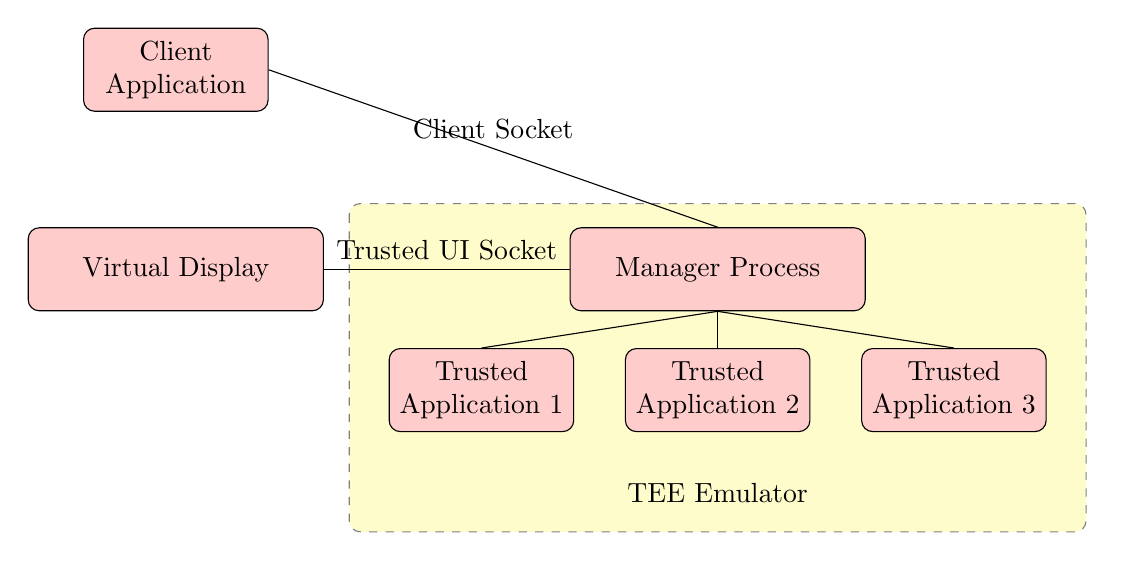
\begin{tikzpicture}
    \node (manager) [process] {Manager Process};
    \path (manager.south)+(-3.0,-1.0) node (ta1) [ta] {Trusted Application 1};
    \path (manager.south)+(0.0,-1.0) node (ta2) [ta] {Trusted Application 2};
    \path (manager.south)+(3.0,-1.0) node (ta3) [ta] {Trusted Application 3};

    \path [draw, -] (ta1.north) -- node [above] {} (manager.south);
    \path [draw, -] (ta2.north) -- node [above] {} (manager.south);
    \path [draw, -] (ta3.north) -- node [above] {} (manager.south);

    \path (manager.south) +(0,-\blockdist) node (teeemu) {TEE Emulator};

    \begin{pgfonlayer}{background}
        % a and b are corner nodes for the rectangle later
        \path (ta1.west |- manager.north)+(-0.5,0.3) node (a) {};
        \path (ta3.east |- teeemu.east)+(+0.5,-0.5) node (b) {};

        % Draw a nice yellow rectangle on background layer
        \path[fill=yellow!20,rounded corners, draw=black!50, dashed]
            (a) rectangle (b);
    \end{pgfonlayer}

    \path (manager.west)+(-5.0,0.0) node (virtuald) [process] {Virtual Display};
    \path (virtuald.north)+(0.0,2.0) node (ca) [ta] {Client Application};

    \path [draw, -] (virtuald.east) -- node [above] {Trusted UI Socket} (manager.west);
    \path [draw, -] (ca.east) -- node [above] {Client Socket} (manager.north);
\end{tikzpicture}
\caption{Block diagram for top-level architecture of Trusted User Interface API
         implementation in Open-TEE}
\label{fig:architecture_block_diagram}
\end{figure}
